\chapter{A Template chapter}
\label{chapter:example_chapter}

This chapter contains some examples of how to use equations, tables and figures in the template. The last section shows how it all comes together in the final document.


\section{Equations}

%%%%%%%%%%%%%%%%%%%%%%%%%%%%%%%%%%%%%%%%%%%%%%%%%%%%%%%%%%%%
\subsection*{Single line equations}
%%%%%%%%%%%%%%%%%%%%%%%%%%%%%%%%%%%%%%%%%%%%%%%%%%%%%%%%%%%%
\vspace{0.4cm}

\begin{equation}
	l = \int ds =  \int_t \sqrt{\left(\frac{dx}{dt} \right)^2 + \left(\frac{dy}{dt} \right)^2 + \left(\frac{dz}{dt} \right)^2} dt \; .
	\label{eq:curve_length_3D_cartesian}
\end{equation}

\vspace{0.4cm}

\begin{equation}
	ds^2 = -\left( 1 - \frac{2 M}{ r}  \right)  dt^2 + \left( 1 - \frac{2 M}{ r}  \right)^{-1} dr^2 + r^2 d \theta^2 + r^2 \sin^2 \theta d \phi^2
	\label{eq:schwarzschild_solution}
\end{equation}

\vspace{0.4cm}

\begin{equation}
	\rho = \rho_0 + \epsilon \rho_1 \qquad p = p_0 + \epsilon p_1 \qquad \psi = \psi_0 + \epsilon \psi_1 \; .
	\label{eq:linear_perturbations}
\end{equation}

\vspace{0.4cm}

%%%%%%%%%%%%%%%%%%%%%%%%%%%%%%%%%%%%%%%%%%%%%%%%%%%%%%%%%%%%
\subsection*{Single line equations with text}
%%%%%%%%%%%%%%%%%%%%%%%%%%%%%%%%%%%%%%%%%%%%%%%%%%%%%%%%%%%%

\vspace{0.4cm}

\begin{equation}
	\lambda_B \sim \SI{0.5}{kpc} \left( \frac{ 10^{-22} \; \text{eV} }{m} \right) \left( \frac{ 250 \; \text{km/s} }{v} \right) \;.
\end{equation}

\vspace{0.4cm}

%%%%%%%%%%%%%%%%%%%%%%%%%%%%%%%%%%%%%%%%%%%%%%%%%%%%%%%%%%%%
\subsection*{Single line equations with box}
%%%%%%%%%%%%%%%%%%%%%%%%%%%%%%%%%%%%%%%%%%%%%%%%%%%%%%%%%%%%

\vspace{0.4cm}

\begin{equation}
		\boxed{
				T_{\text{Scalar}}^{\mu \nu} = 
				(g^{\mu \alpha}g^{\nu \beta} + g^{\mu \beta}g^{\nu \alpha} - g^{\mu \nu}g^{\alpha \beta}) \partial_\alpha \Psi \partial_\beta \Psi - g^{\mu \nu} \mu^2 \Psi^2 
		}
	\label{eq:superradiant_condition}
\end{equation}

\begin{equation}
	\boxed{
		\boxed{
			\omega < m \Omega_H
		}
	}
	\label{eq:superradiant_condition_2}
\end{equation}


\vspace{0.4cm}


%%%%%%%%%%%%%%%%%%%%%%%%%%%%%%%%%%%%%%%%%%%%%%%%%%%%%%%%%%%%
\subsection*{Multiline equations}
%%%%%%%%%%%%%%%%%%%%%%%%%%%%%%%%%%%%%%%%%%%%%%%%%%%%%%%%%%%%

\vspace{0.4cm}

\begin{equation}
	\begin{aligned}
		a 		&= J/M \\
		\rho 	&= r^2 + a^2 \cos^2 \theta  \\
		\Delta	&= r^2 - 2 M r + a^2 \; .
	\end{aligned}
\end{equation}

\vspace{0.4cm}

\begin{equation}
	\begin{aligned}
		\left[  \frac{(r^2 + a^2)}{\Delta} - a^2 \sin^2 \theta\right]\frac{\partial^2 \Psi}{\partial t^2} + \frac{4M a r}{\Delta} &\frac{\partial^2 \Psi}{\partial t \partial \varphi} + \left[ \frac{a^2}{\Delta} - \frac{1}{\sin^2 \theta}\right] \frac{\partial^2 \Psi}{\partial \varphi^2} + \\[10pt] & - \frac{\partial}{\partial r} \left( \Delta \frac{\partial  \Psi}{\partial r}\right) - \frac{1}{\sin \theta} \frac{\partial}{\partial t}\left( \sin \theta \frac{\partial \Psi}{\partial \theta}\right) = 0 \; .
	\end{aligned}
\end{equation}

\vspace{0.4cm}

\begin{equation}
	\begin{aligned}
		\sum_{m} \mathcal{A}_{+}^{m}&\left[ \phi_m^+ - i \tilde{Z}_0 \left(\phi_m^+\right)'   \right] + \mathcal{A}_{-}^{m}\left[ \phi_m^- - i \tilde{Z}_0 \left(\phi_m^-\right)'   \right] = \\
		=&\sum_{m} \epsilon \left(\frac{i  \tilde{Z}}{2}\right) \left[ \mathcal{A}_{+}^{m} \left(\phi_m^+\right)' + \mathcal{A}_{+}^{m+2} \left(\phi_{m+2}^+\right)' + \mathcal{A}_{+}^{m-2} \left(\phi_{m-2}^+\right)'  \right] + \\
		& \qquad +\sum_{m} \epsilon \left(\frac{i  \tilde{Z}}{2}\right) \left[ \mathcal{A}_{-}^{m} \left(\phi_m^-\right)' + \mathcal{A}_{-}^{m+2} \left(\phi_{m+2}^-\right)' + \mathcal{A}_{-}^{m-2} \left(\phi_{m-2}^-\right)'  \right] \; ,
	\end{aligned}
	\label{eq:infinite_set_of_equations}
\end{equation}
%

\vspace{0.4cm}

%%%%%%%%%%%%%%%%%%%%%%%%%%%%%%%%%%%%%%%%%%%%%%%%%%%%%%%%%%%%
\subsection*{Matrix Equations}
%%%%%%%%%%%%%%%%%%%%%%%%%%%%%%%%%%%%%%%%%%%%%%%%%%%%%%%%%%%%
\vspace{0.4cm}

\begin{equation}
	\arraycolsep = 5pt \def\arraystretch{1.1}
	\left[
	\begin{array}{ccccccc}
		\ddots    &  \beta_+^4  &               &               &               &               &             \\
		\beta_+^6 & \Lambda_+^4 &  \beta_+^2  &               &               &               &             \\
		&  \beta_+^4  & \Lambda_+^2 &  \beta_+^0  &               &               &             \\
		&               &  \beta_+^2  & \Lambda_+^0 &  \beta_+^2  &               &             \\
		&               &               &  \beta_+^0  & \Lambda_+^2 &  \beta_+^4  &             \\
		&               &               &               &  \beta_+^2  & \Lambda_+^4 & \beta_+^6 \\
		&               &               &               &               &  \beta_+^4  &   \ddots
	\end{array} 
	\right]
	\left[
	\begin{array}{c}
		\vdots \\
		\mathcal{A}_{+}^{-4} \\
		\mathcal{A}_{+}^{-2} \\
		\mathcal{A}_{+}^{0} \\
		\mathcal{A}_{+}^{2} \\
		\mathcal{A}_{+}^{4} \\
		\vdots
	\end{array} 
	\right]
	=
	\left[
	\begin{array}{c}
		\vdots \\
		0 \\
		-\beta_-^0 \\
		-\Lambda_-^0 \\
		-\beta_-^0 \\
		0 \\
		\vdots
	\end{array} 
	\right]
	\label{eq:matrix_eigenvalue_equation}
\end{equation}

%%%%%%%%%%%%%%%%%%%%%%%%%%%%%%%%%%%%%%%%%%%%%%%%%%%%%%%%%%%%
\subsection*{Conditional equation}
%%%%%%%%%%%%%%%%%%%%%%%%%%%%%%%%%%%%%%%%%%%%%%%%%%%%%%%%%%%%

\vspace{0.4cm}

\begin{equation}
	\alpha(t , \mathbf{r}) = 
	\begin{cases}
		\alpha_0 \qquad \text{if} \qquad (\mathbf{r} -\mathbf{R_{orbit})}^2 < R_a^2 \\
		\alpha_0 \qquad \text{if} \qquad (\mathbf{r} +\mathbf{ R_{orbit})}^2 < R_a^2 \\
		0   \; \;\qquad \text{otherwise}
		\label{eq:alpha_binary_bh}
	\end{cases} \; ,
\end{equation}

\vspace{0.4cm}

\section{Tables}

\begin{table}[h]
	\caption{Example table number 1}
	\label{table:an_example_table}
	\centering
	\begin{tabular}{clllll}
		\toprule
		\midrule[0.4pt]
		ID&$A$  & $r_0$  &  $\sigma$ &  $\omega$  &  $m$  \\
		\midrule
		S1 & 3.5 & 40.0 & 4.0 & 1.28 & 0 \\
		S2 & 3.5 & 15.0 & 2.0 & 0.1 & 2 \\
		\bottomrule
	\end{tabular}
\end{table}


\begin{table}[h!]
	\centering
	\caption{Example table number 2}
	\begin{tabular}{SSSSSSS}
		\toprule
		\midrule[0.4pt]
		{$k$} & {$J_0(x)$} & {$J_1(x)$} & {$J_2(x)$} & {$J_3(x)$} & {$J_4(x)$} & {$J_5(x)$} \\ 
		\midrule
		1     & 2.4048     & 3.8317     & 5.1356     & 6.3802     & 7.5883     & 8.7715     \\
		2     & 5.5201     & 7.0156     & 8.4172     & 9.7610     & 11.0647    & 12.3386    \\
		3     & 8.6537     & 10.1735    & 11.6198    & 13.0152    & 14.3725    & 15.7002    \\
		4     & 11.7915    & 13.3237    & 14.7960    & 16.2235    & 17.6160    & 18.9801     \\ 
		\midrule[0.4pt]
		\bottomrule
	\end{tabular}
	\label{table:bessel_zeros}
\end{table}

\section{Figures}

Generating figures in a consistent manner is usually challenge. Especially when the work to be presented is made by a team of several elements. The graphics presented in this template are generated with the \href{"aa"}{\texttt{Jlop}} template in python. 

\subsection*{Single Figure}

\begin{figure}[!ht]
	\centering
	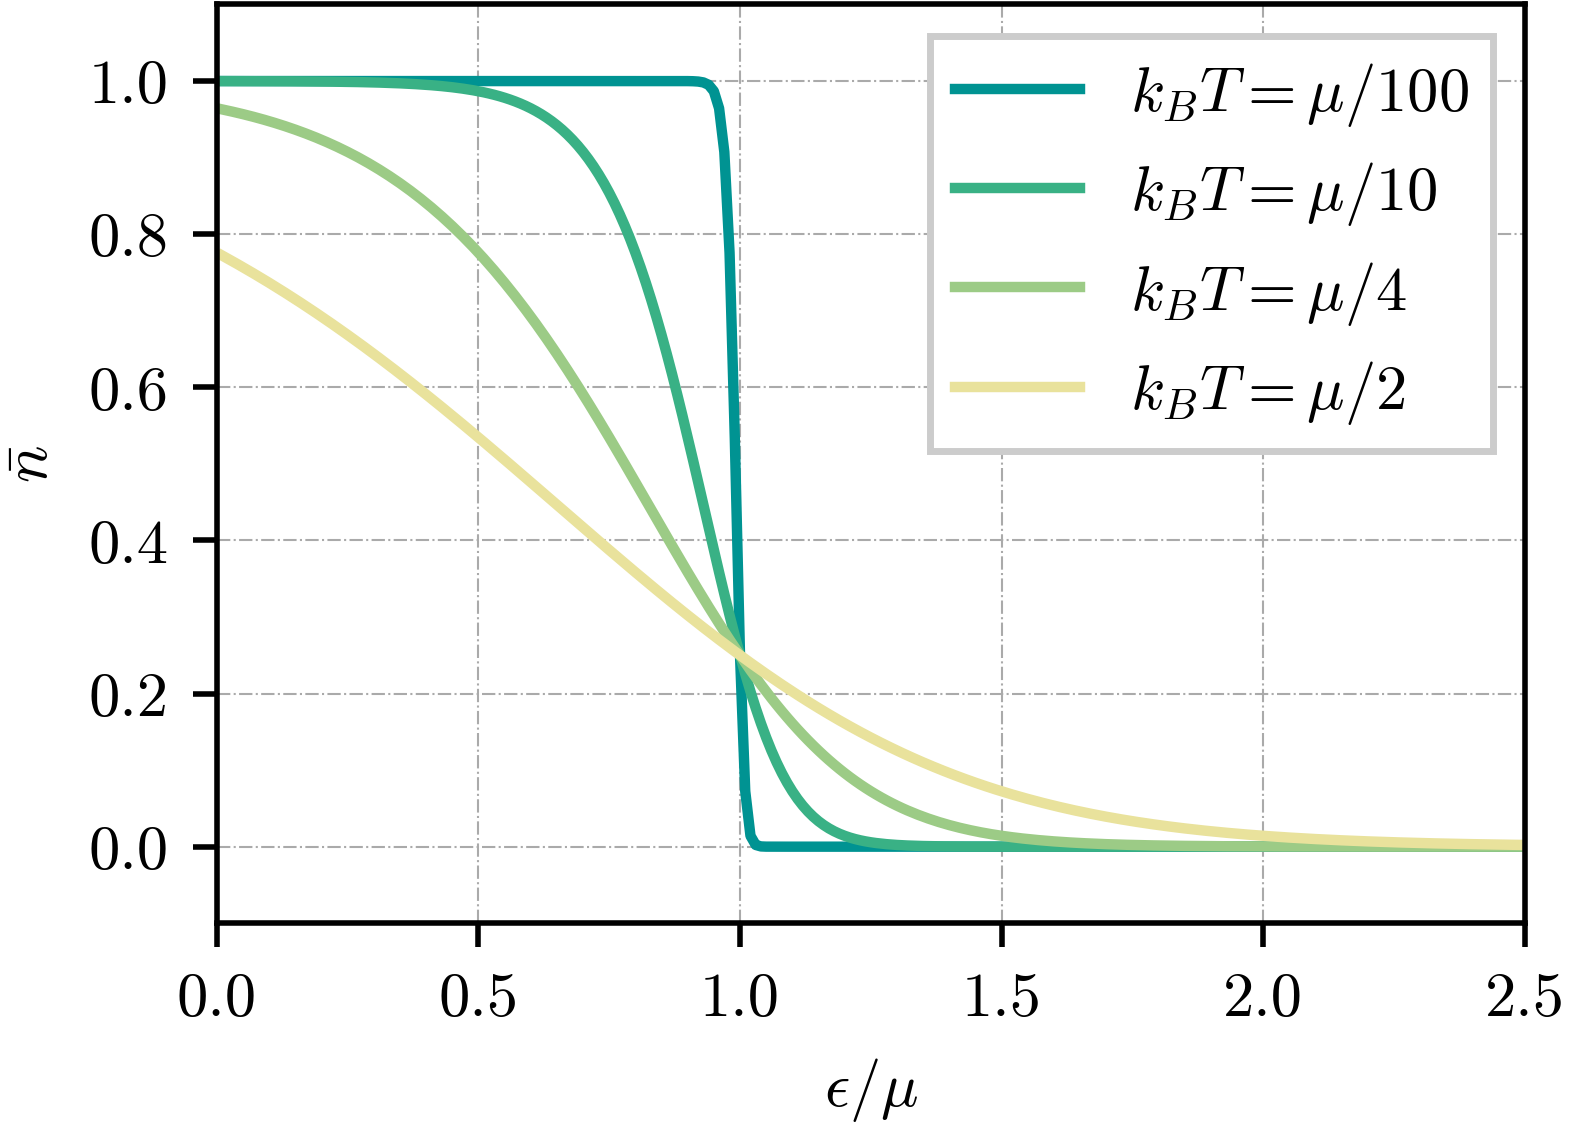
\includegraphics{figures/chapter_B/jlop_sc_sqroot.png}
	\caption{An example figure}
	\label{fig1:single_image}
\end{figure}

\pagebreak
\subsection*{Side By Side}

\begin{figure}[!ht]
	\centering
	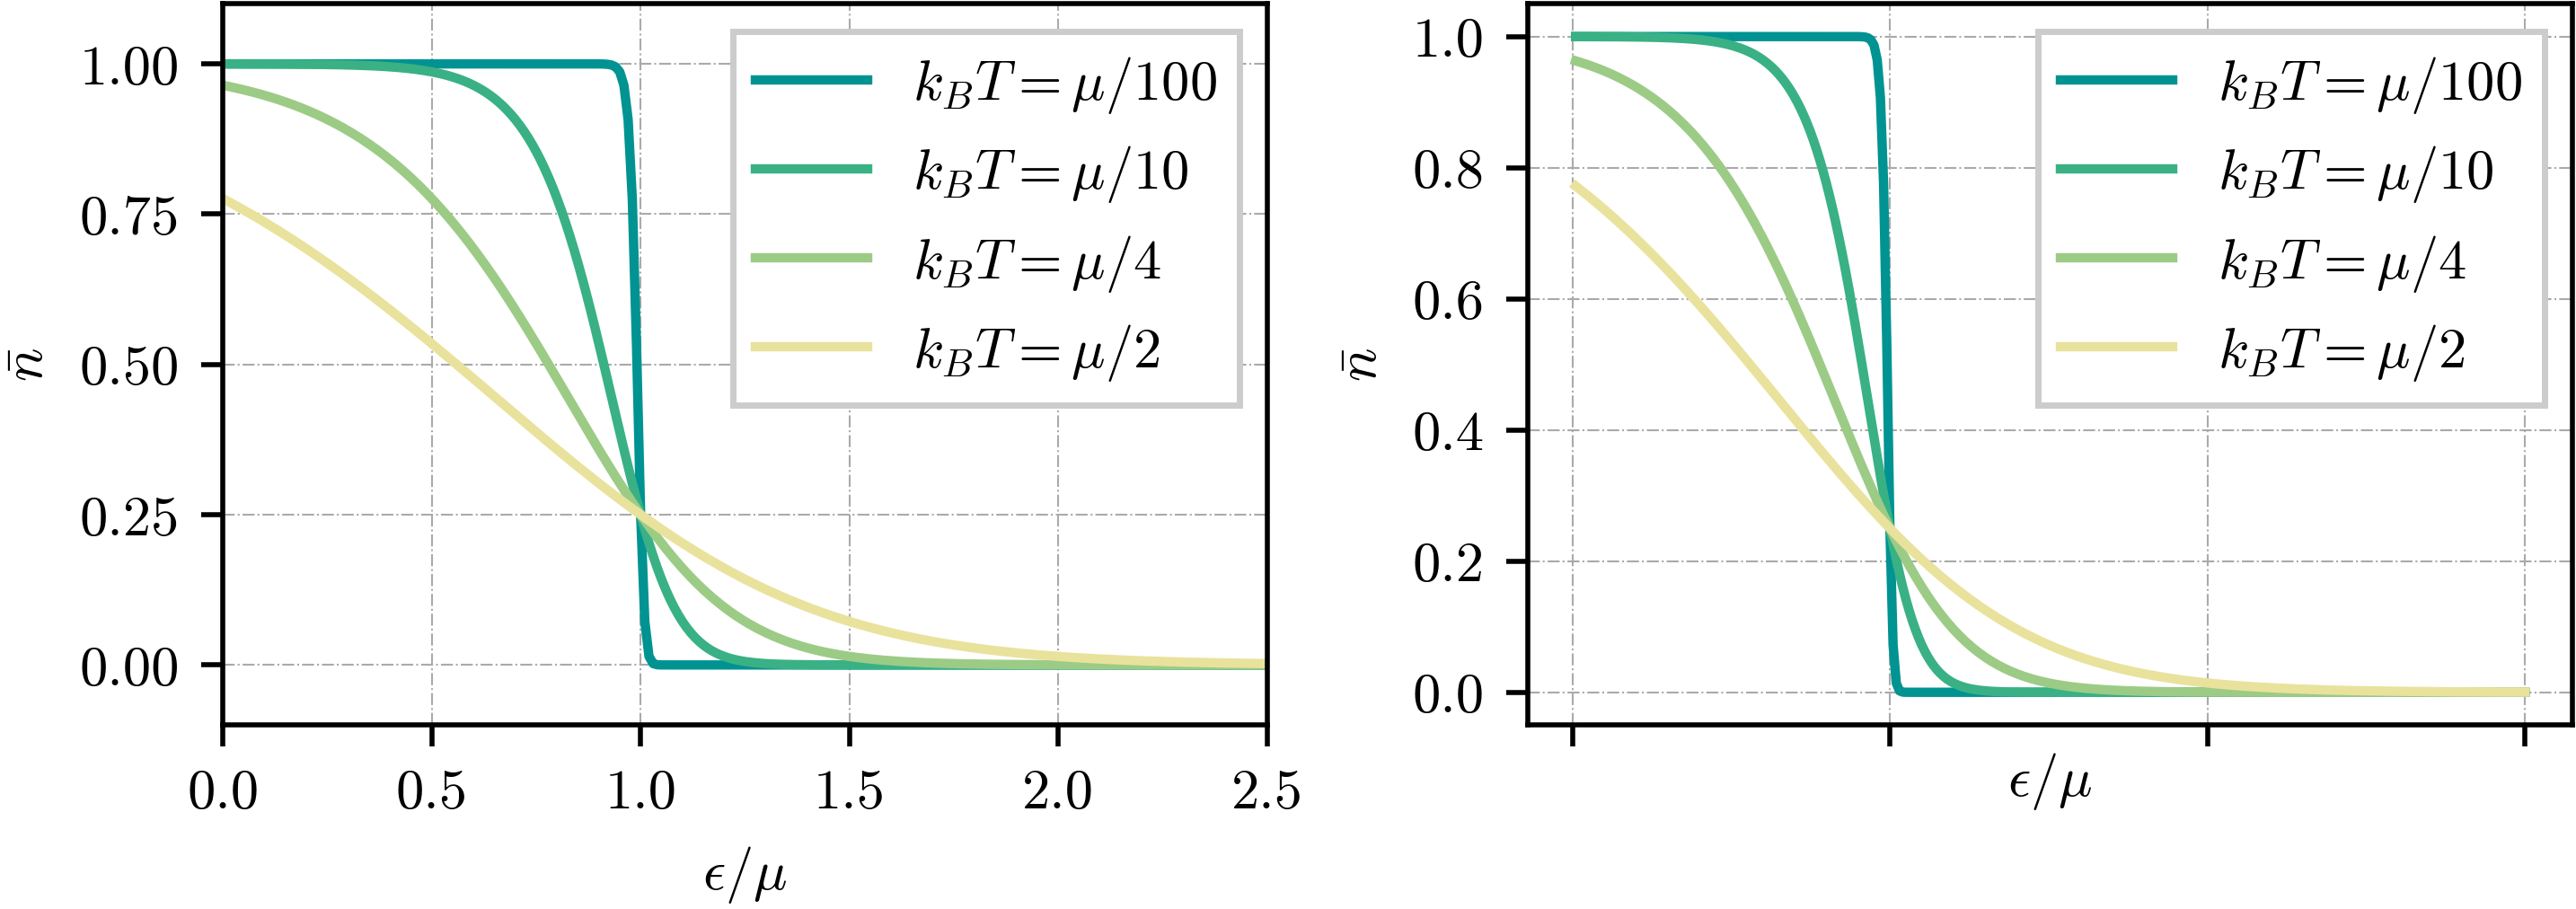
\includegraphics{figures/chapter_B/jlop_dc_golden.png}
	\caption{An example figure with two elements. The two plots where generated as a single image with the correct document width. If this is not possible, follow the procedure done to generate figure \ref{fig1:side_by_side_image}.}
	\label{fig1:side_by_side_single}
\end{figure}


\begin{figure}[h!]
	\centering
	\includegraphics[width=.48\linewidth]{example-image-a}
	\includegraphics[width=.48\linewidth]{example-image-b}
	\caption{An example figure with two elements. It is usually better to make a single image with both plots as to input a single file. When that is not possible, one should resort to this method}
	\label{fig1:side_by_side_image}
\end{figure}

\vfill
\pagebreak
\section{Putting it al together}

\lipsum[5]

\begin{equation}
	\lambda_B \sim \SI{0.5}{kpc} \left( \frac{ 10^{-22} \; \text{eV} }{m} \right) \left( \frac{ 250 \; \text{km/s} }{v} \right) \;.
\end{equation}

\lipsum[10]

\begin{table}[h]
	\caption{Example table number 1}
	\label{table:example_table_2}
	\centering
	\begin{tabular}{clllll}
		\toprule
		\midrule[0.4pt]
		ID&$A$  & $r_0$  &  $\sigma$ &  $\omega$  &  $m$  \\
		\midrule
		S1 & 3.5 & 40.0 & 4.0 & 1.28 & 0 \\
		S2 & 3.5 & 15.0 & 2.0 & 0.1 & 2 \\
		\bottomrule
	\end{tabular}
\end{table}

\lipsum[2]

\begin{figure}[t!]
	\centering
	\includegraphics[width=.48\linewidth]{example-image-a}
	\includegraphics[width=.48\linewidth]{example-image-b}
	\caption{An example figure with two elements. It is usually better to make a single image with both plots as to input a single file. When that is not possible, one should resort to this method}
	\label{fig1:side_by_side_image_2}
\end{figure}

\lipsum